\documentclass[12pt,a4paper]{article}
\usepackage[utf8]{inputenc}
\usepackage[T1]{fontenc}
\usepackage{amsmath}
\usepackage{amsfonts}
\usepackage{amssymb}
\usepackage{graphicx}
\usepackage{subfigure}
\usepackage{float}
\usepackage{caption}
\DeclareMathOperator{\xyz}{\textbf{numpy.random.normal()}}
\title{CS 331: Stochastic Gradient Descent Methods Assignment 2}
\author{Lukang Sun, ID: 182056}
\begin{document}
	\maketitle
	\paragraph{p1.}
	(1.)\begin{equation*}
		\frac{||a||^2}{t}+t||b||^2+2\langle a,b\rangle = ||\frac{a}{\sqrt{t}}+\sqrt{t}b||^2\geq 0,
	\end{equation*}
	this proves 
	
	\begin{equation}
		\langle a,b\rangle\leq \frac{||a||^2}{2t}+\frac{t||b||^2}{2}.
	\end{equation}
	
	(2.)
	\begin{equation*}
		||a+b||^2=||a||^2+||b||^2+2\langle a,b\rangle,
	\end{equation*}
		since $2\langle a,b\rangle\leq ||a||^2+||b||^2$, we have finally
		\begin{equation}
			||a+b||^2\leq 2||a||^2+2||b||^2
		\end{equation}
	
	(3.)
	from inequality(2), we know
	\begin{equation*}
		||a||^2=||a+b-b||^2\leq 2||a+b||^2+2||-b||^2=2||a+b||^2+2||b||^2,
	\end{equation*}
	 move $2||b||^2$ to the left hand side, then both sides time 0.5, we have 
	 \begin{equation}
	 	\frac{1}{2}||a||^2-||b||^2\leq ||a+b||^2
	 \end{equation}
 
 \paragraph{p2.}
  if $C=0$, then we have 
  \begin{equation*}
  	\mathbb{E}[||x^k-x^*||^2]\leq (1-\gamma \mu)^k||x_0-x^*||^2,
  \end{equation*}
combine Markov inequality, for any $\varepsilon>0,$ we then have 
\begin{equation*}
	\begin{aligned}
		\lim _{k \rightarrow \infty} \operatorname{Prob}\left(\left\|X^{k}-X\right\|>\varepsilon\right)=\lim _{k \rightarrow \infty} \operatorname{Prob}\left(\left\|X^{k}-X\right\|^2>\varepsilon^2\right)& \leq 	\lim _{k \rightarrow \infty}\frac{\mathbb{E}[||x^k-x^*||^2]}{\varepsilon^2}\\
		&\leq \lim_{k \rightarrow \infty}\frac{(1-\gamma \mu)^k||x_0-x^*||^2}{\varepsilon^2}=0.\\
	\end{aligned}
\end{equation*}

\paragraph{p3.}
denote $r^{k}=x^k-x^*$
\begin{equation}
	\begin{aligned}
		\mathbb{E}[||r^{k+1}||^2\mid x^k]&\leq||r^k||^2+2\gamma\langle \nabla f(x^k)-\nabla f(x^*),x^k-x^*\rangle+\gamma^2||\nabla f(x^k)-\nabla f(x^*)||^2+\gamma^2\sigma^2\\
		&\leq (1-\frac{2\gamma\mu L}{\mu+L})||r^k||^2-\gamma(\gamma-\frac{2}{\mu+L})||\nabla f(x^k)-\nabla f(x^*)||^2+\gamma^2\sigma^2,
	\end{aligned}
\end{equation}
where the second inequality uses 
\begin{equation*}
	\langle\nabla f(x)-\nabla f(y), x-y\rangle\geq \frac{\mu L}{\mu+L}||x-y||^2+\frac{1}{\mu+L}||\nabla f(x)-\nabla f(y)||^2.
\end{equation*}
 We set $\gamma =\frac{2(1+\frac{\mu}{L})}{L(1+3\frac{\mu}{L})}$, then $\gamma\leq \frac{2}{L}\frac{1}{1+\frac{2\frac{\mu}{L}}{1+\frac{\mu}{L}}}\leq \frac{2}{L}\frac{1}{1+\frac{\mu}{L}}=\frac{2}{L+\mu},$ since $\frac{2}{1+\frac{\mu}{L}}\geq 1$. We insert this $\gamma$ into (4), take whole expectation then we have 
 \begin{equation}
 	\mathbb{E}[||r^{k+1}||^2]\leq (1-\frac{4}{3+\frac{L}{\mu}})\mathbb{E}[||r^k||^2]+\gamma^2\sigma^2,
 \end{equation}
use (5) iteratively for k from 0 to $i-1$, then we have 

\begin{equation*}
	\mathbb{E}[||r^{i}||^2]\leq (1-\frac{4}{3+\frac{L}{\mu}})^i||r^0||^2+\frac{\gamma^2\sigma^2}{\frac{2\gamma \mu L}{\mu+L}}\leq (1-\frac{4}{3+\frac{L}{\mu}})^i||r^0||^2+\frac{\gamma\sigma^2}{\mu},
\end{equation*}
the second inequality uses $\frac{\mu+L}{2L}\leq 1.$ So in order to make  $(1-\frac{4}{3+\frac{L}{\mu}})^k\leq \epsilon$, we only need
\begin{equation*}
	k\geq \frac{\frac{L}{\mu}+3}{4}\log(\frac{1}{\epsilon}),
\end{equation*}
finally, we reach
\begin{equation*}
	\mathbb{E}[||x^k-x^*||^2]\leq \epsilon||x^0-x^*||^2+\frac{\gamma\sigma^2}{\mu}.
\end{equation*}

\paragraph{p4.}
In my first set of experiments(see Figure \ref{img1}.), $A = \left [
\begin{array}{cc}
	0.02 & 0 \\
	0 & 2
\end{array}
\right ], d = 2, x^0 = (5,5), L = 2, \mu = 0.02, \gamma = \frac{2(1+\frac{\mu}{L})}{L(1+3\frac{\mu}{L})}\approx 0.9806, \epsilon = 10^{-10}, \frac{\frac{L}{\mu}+3}{4}\log(\frac{1}{\epsilon})\approx 595, k=1485, $  I set  $\sigma$ equals 0.1, 0.2, 0.01, 0.05, 0.001, 0.005 separately, to estimate $\mathbb{E}\left[||x^k-x^*||^2\right]$, I sample $x^k$ for 100 times and take the average value of $||x^k-x^*||^2$, I will denote the average value as $E$ and $\frac{\gamma\sigma^2}{\mu}$ as $T$ in the results. I use $\xyz$to generate $\xi.$

\begin{figure}
	\centering
	\subfigure[$\gamma = 0.9806,\sigma = 0.2$  ]{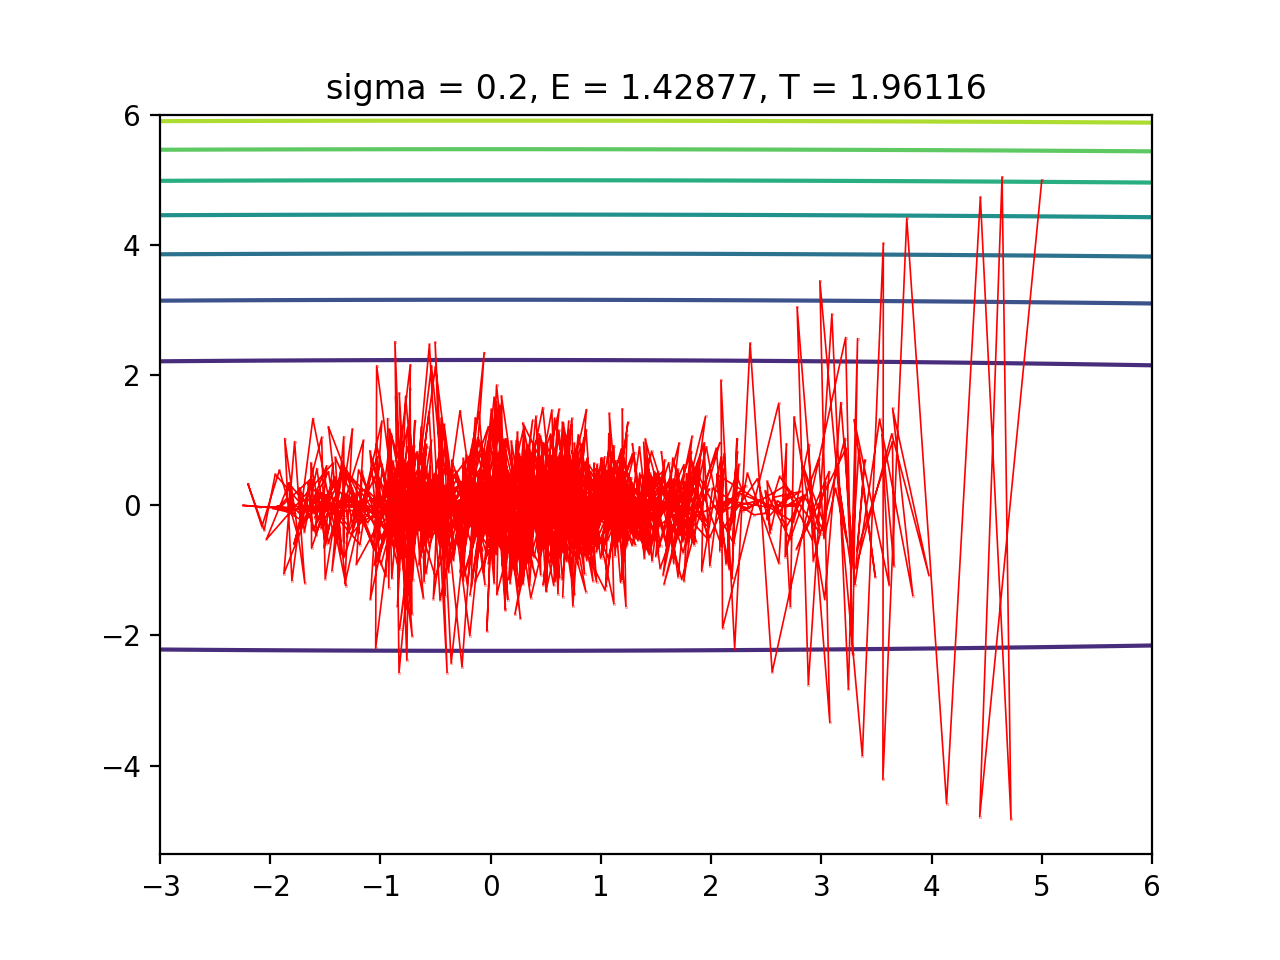
\includegraphics[width=6.7cm]{Figure_7.png}} 
	\subfigure[$\gamma = 0.9806,\sigma = 0.1$]{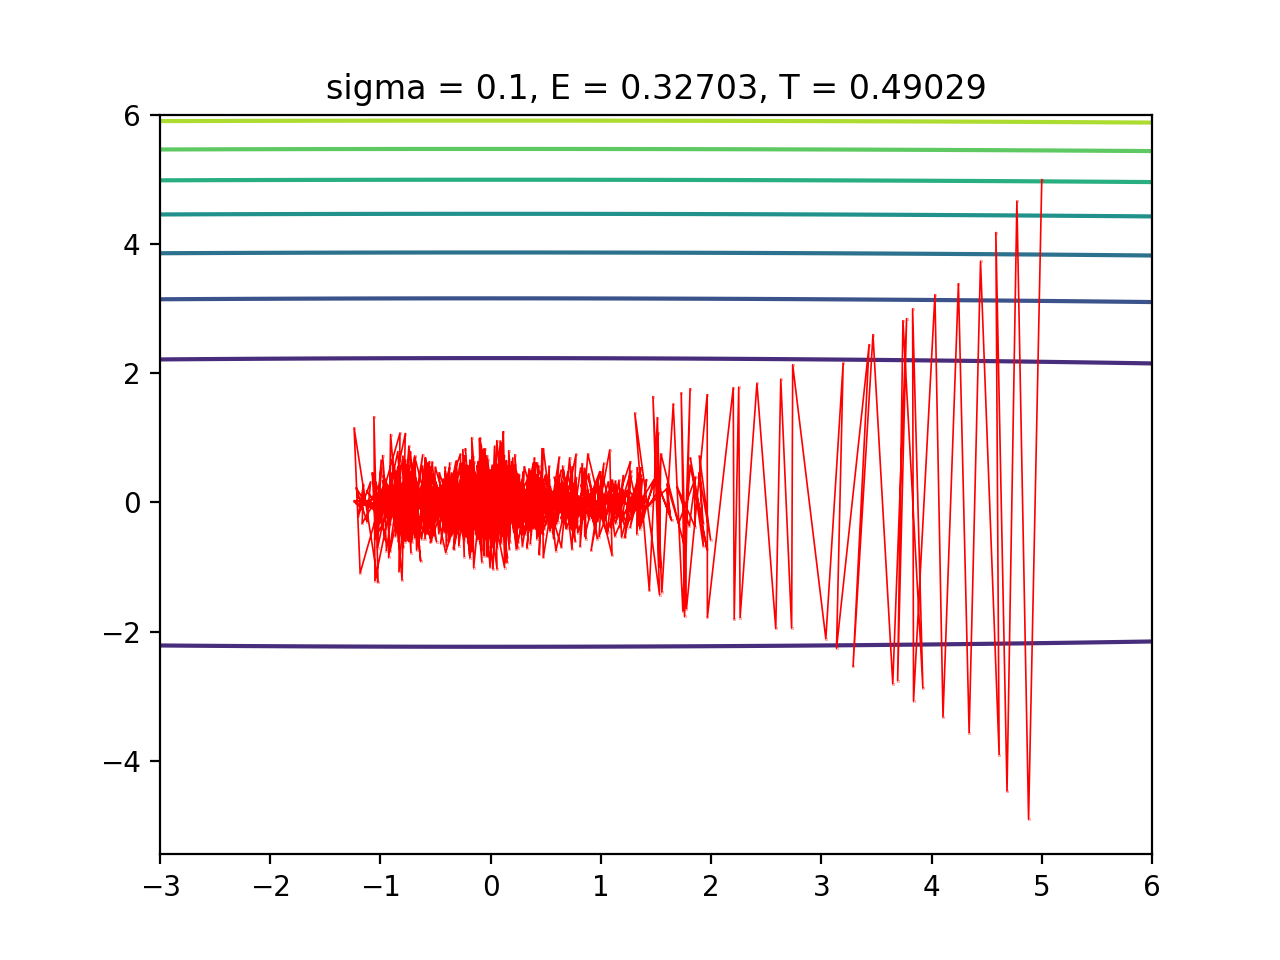
\includegraphics[width=6.7cm]{Figure_6.png}}
	\\ %换行
	\centering
	\subfigure[$\gamma = 0.9806,\sigma = 0.05 $]{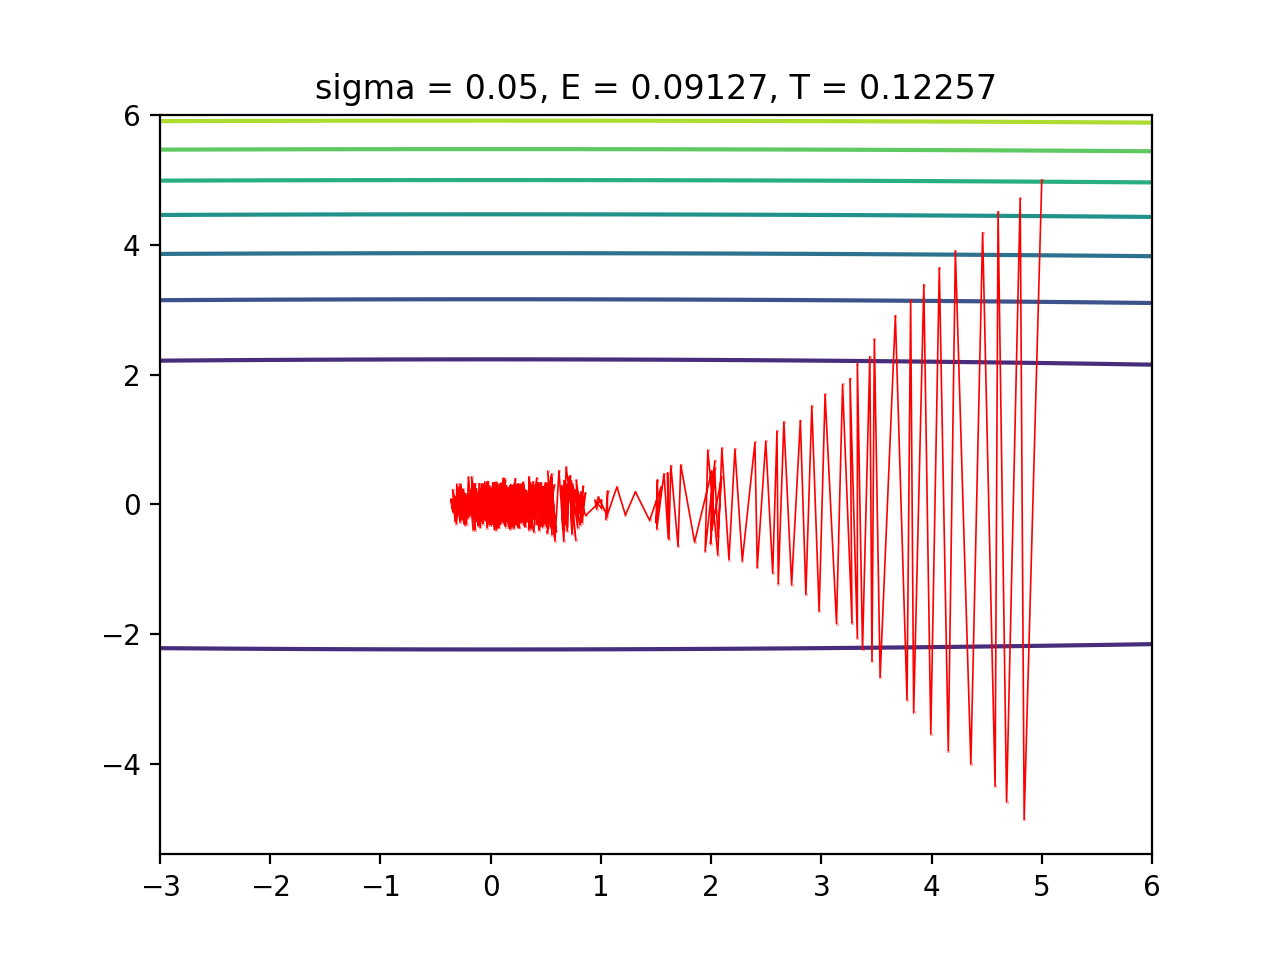
\includegraphics[width=6.7cm]{Figure_3.png}}
	\subfigure[$\gamma = 0.9806,\sigma = 0.01$]{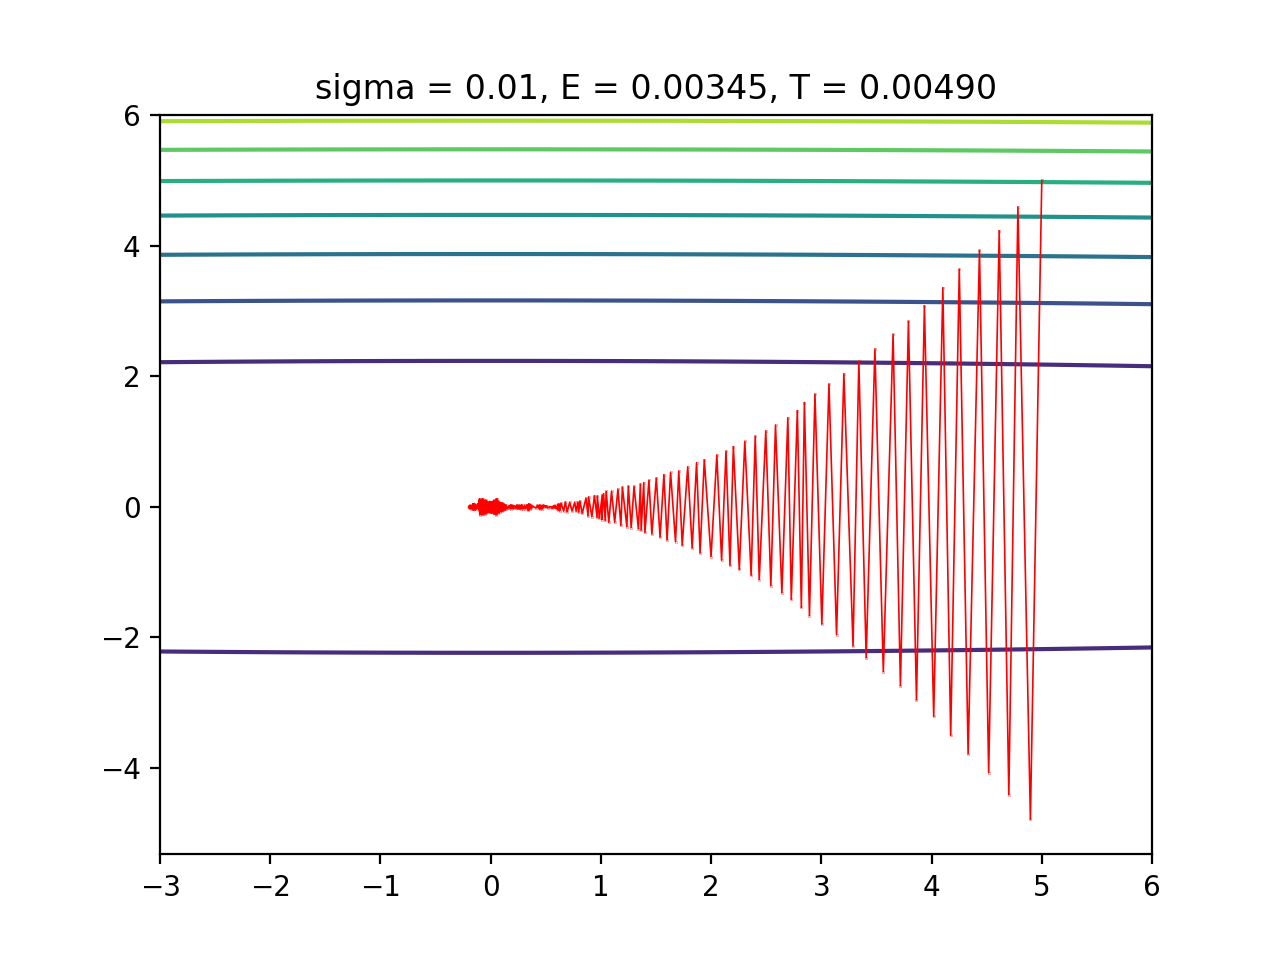
\includegraphics[width=6.7cm]{Figure_2.png}}
	\\
	\centering
	\subfigure[$\gamma = 0.9806,\sigma = 0.005 $]{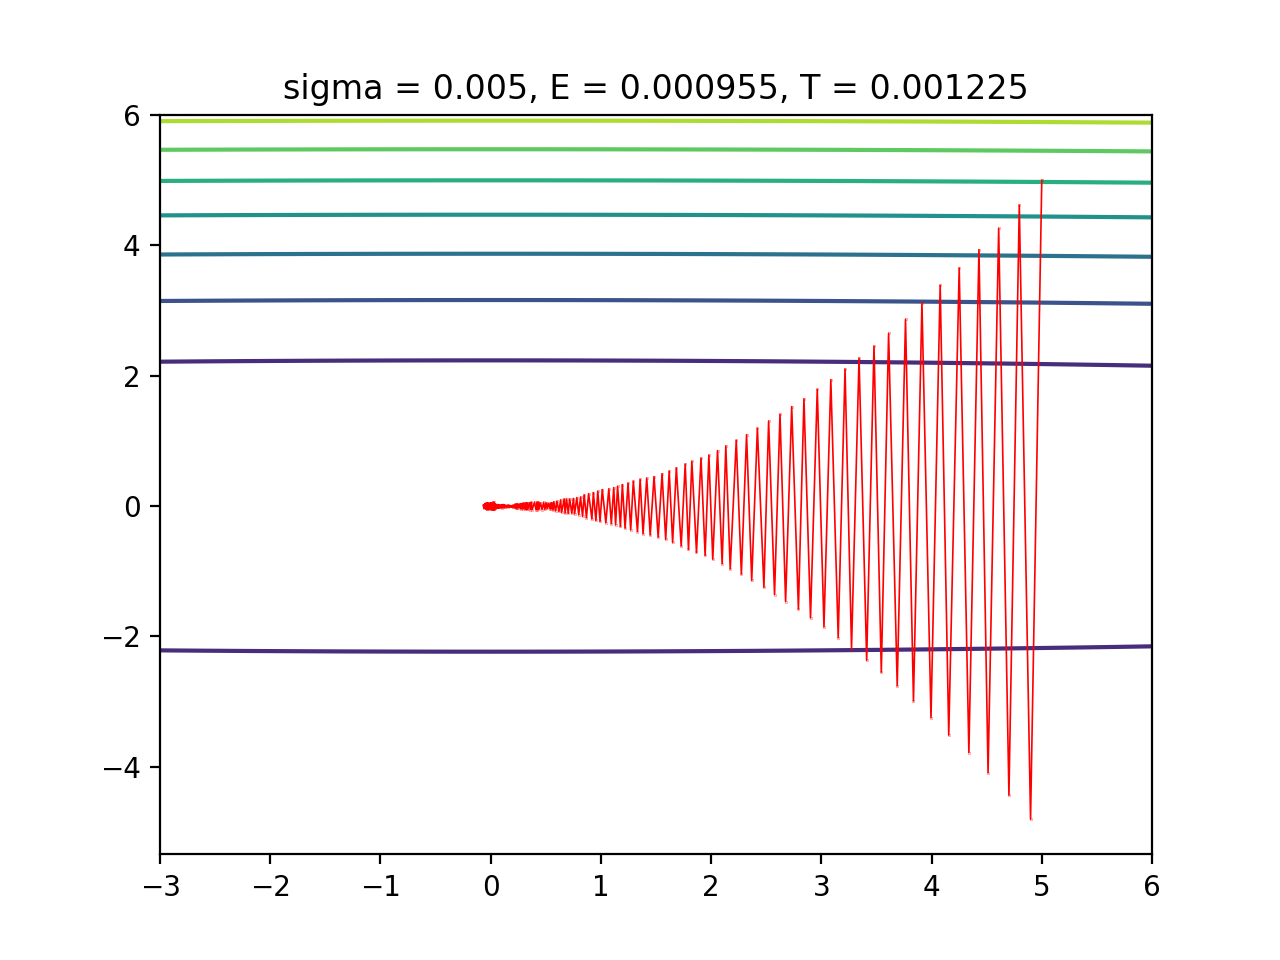
\includegraphics[width=6.7cm]{Figure_4.png}}
	\subfigure[$\gamma = 0.9806,\sigma = 0.001$]{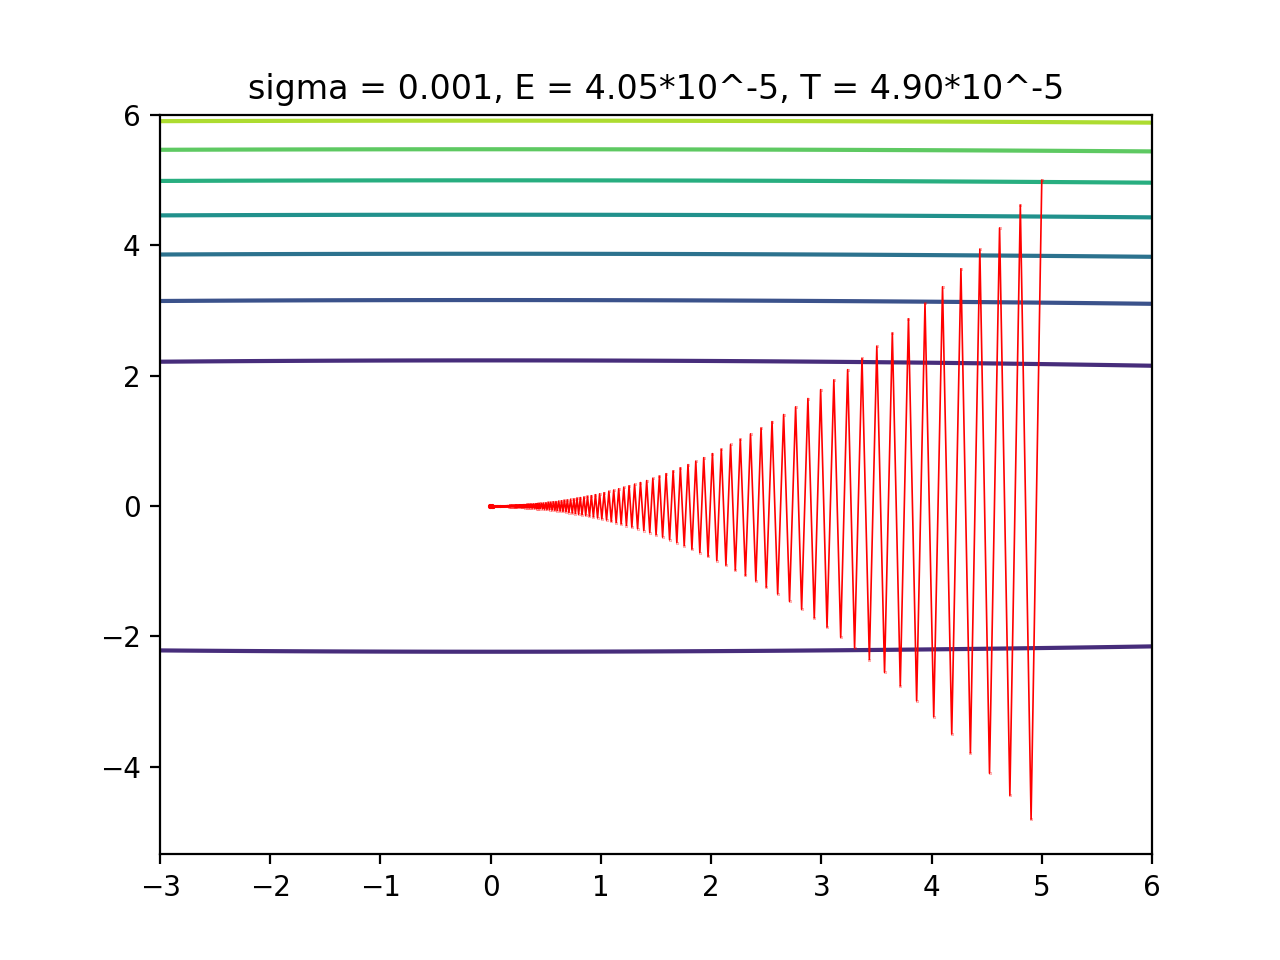
\includegraphics[width=6.7cm]{Figure_5.png}}
	
	\caption{Experiments with different $\sigma$ values, the horizontal axis is $x-axis$ and vertical axis is $y-axis$, the red trajectories show how SGD converges. From the results you can see that $E$ and $T$ always have same magnitude and have similar value, these testify that after enough iteration, SGD  converges to a neighborhood of the optimal solution, it is hard for SGD to converge further after entering into the neighborhood and the neighborhood's size is well predicted by the theory(since $T$ and $E$ are similar). } %图片标题
	\label{img1}
\end{figure}



In my second set of experiments(see Figure \ref{img2}.), $A = \left [
\begin{array}{cc}
	0.02 & 0 \\
	0 & 2
\end{array}
\right ], d = 2, x^0 = (5,5), L = 2, \mu = 0.02, \sigma = 0.1, \epsilon = 10^{-10}, \frac{\frac{L}{\mu}+3}{4}\log(\frac{1}{\epsilon})\approx 595, k=1485, $  I set  step size $\gamma$ approximately equals 0.9806, 0.4903, 0.24515, 0.16343 separately , to estimate $\mathbb{E}\left[||x^k-x^*||^2\right]$, I sample $x^k$ for 100 times and take the average value of $||x^k-x^*||^2$, I will denote the average value as $E$ and $\frac{\gamma\sigma^2}{\mu}$ as $T$ in the results. I use $\xyz$to generate $\xi.$

\begin{figure}
	\centering
	\subfigure[$\gamma = 0.9806, \sigma = 0.1$  ]{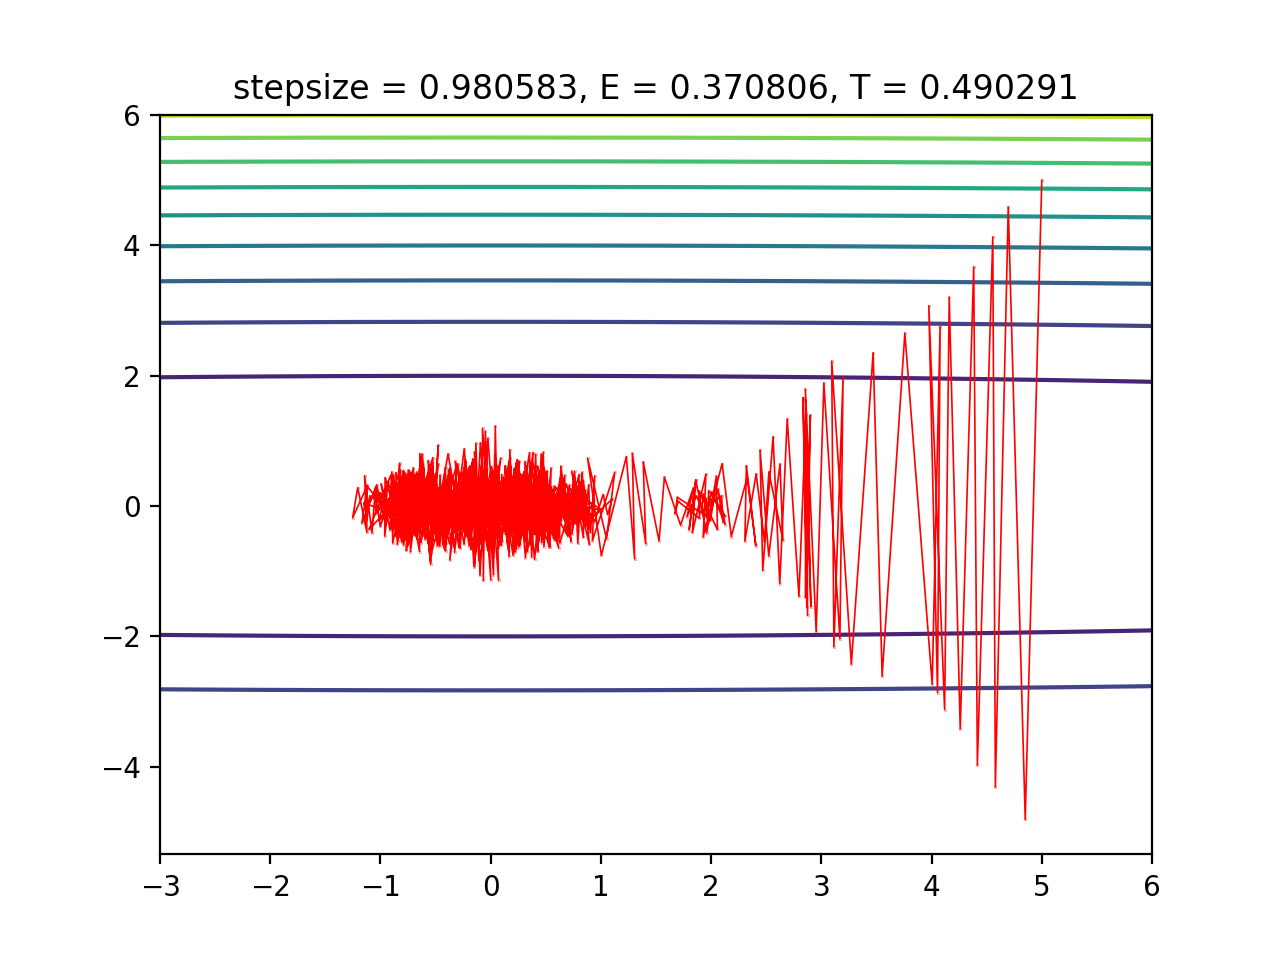
\includegraphics[width=6.7cm]{Figure_11.png}} 
	\subfigure[$\gamma = 0.4903, \sigma = 0.1$]{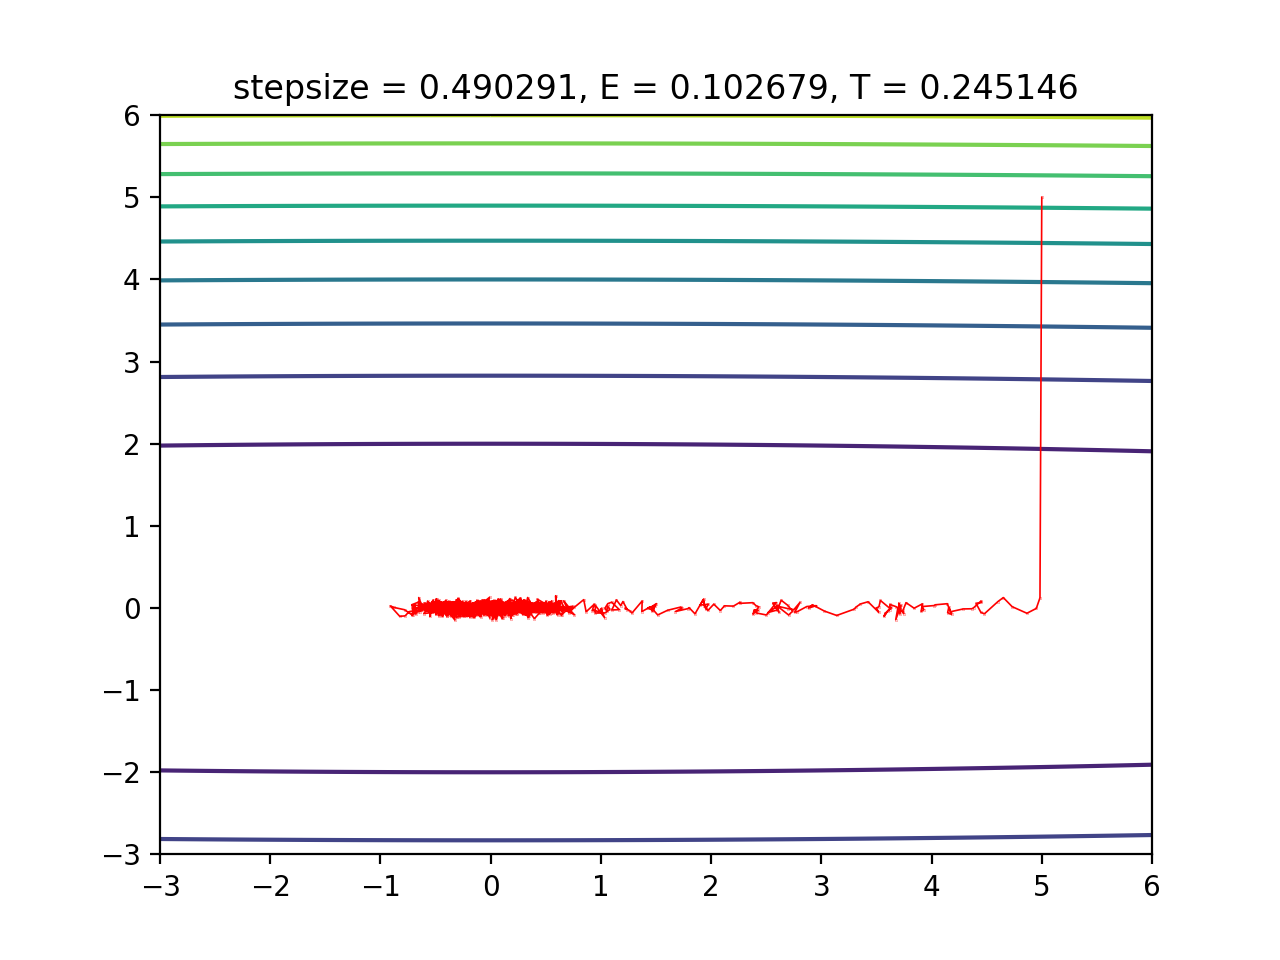
\includegraphics[width=6.7cm]{Figure_12.png}}
	\\ %换行
	\centering
	\subfigure[$\gamma = 0.24515, \sigma = 0.1 $]{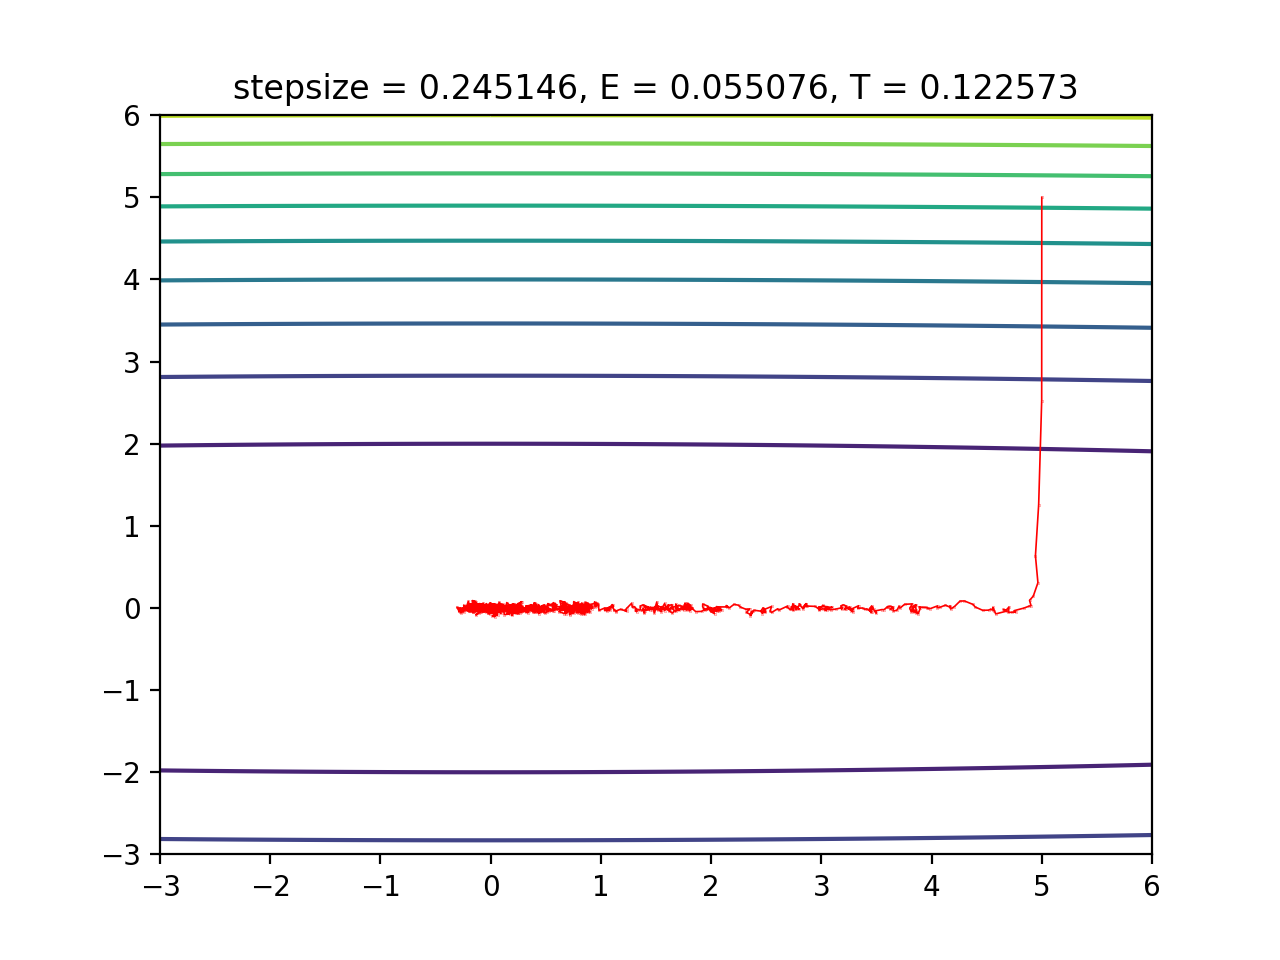
\includegraphics[width=6.7cm]{Figure_13.png}}
	\subfigure[$\gamma = 0.16343, \sigma = 0.1$]{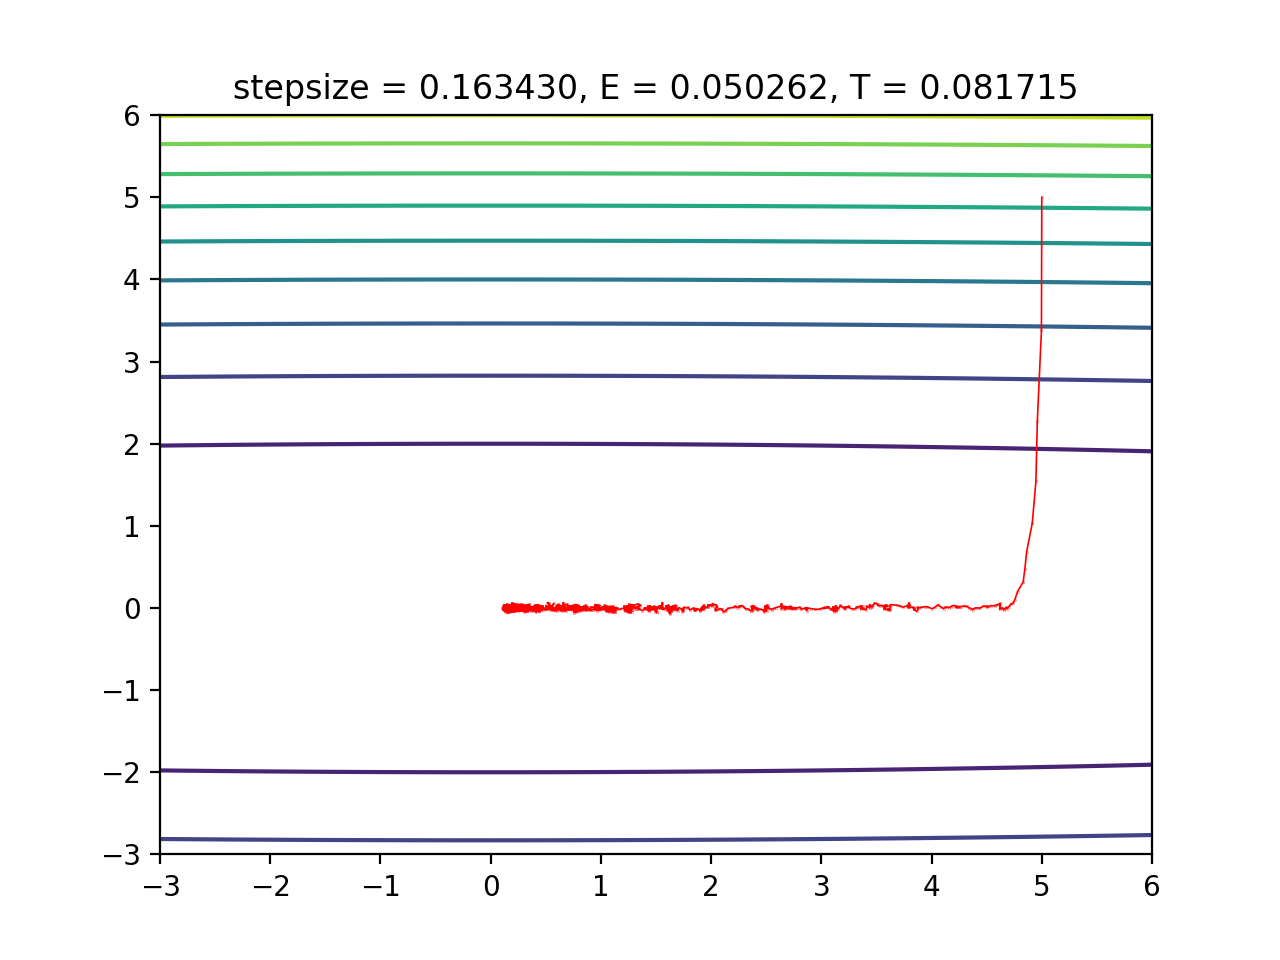
\includegraphics[width=6.7cm]{Figure_14.png}}
	
	\caption{Experiments with different step sizes,  these results testify that the size of the neighborhood has linear growth relationship with step size. From the results, you can also observe  that $\frac{T}{E}\approx 2$, since from the derivation of problem 3., we know the theoretical neighborhood size is $\frac{\gamma^2\sigma^2}{\frac{2\gamma \mu L}{\mu+L}}\approx \frac{1}{2}\frac{\gamma \sigma^2}{\mu}$. } %图片标题
	\label{img2}
\end{figure}



	
\end{document}